%\documentclass[a4paper,12pt]{article}

%% don't forget the document class, generally : \documentclass[a4paper,12pt]{article}

\usepackage[utf8]{inputenc}
\usepackage[french]{babel}
\usepackage{graphicx}
\usepackage{gensymb}
\usepackage{amsmath}
\usepackage{float}
\usepackage{scrextend}
\usepackage{caption} 
\usepackage{siunitx}
\usepackage{enumitem}
\usepackage{amsthm}
\usepackage{fancyhdr}
\usepackage{amssymb}
\usepackage{wrapfig}
\usepackage{geometry}
\usepackage{standalone}
\usepackage{import}
\usepackage[usenames, dvipsnames]{color}

 \usepackage{biblatex} % manages bibliography and references
\addbibresource{sample.bib}


\geometry{hmargin=1in, vmargin=1in}

 \newenvironment{absolutelynopagebreak}
 {\par\nobreak\vfil\penalty0\vfilneg
 \vtop\bgroup}
 {\par\xdef\tpd{\the\prevdepth}\egroup
 \prevdepth=\tpd}
 
 \pagestyle{fancy}                        
\fancyhf{}                               
\fancyhf[HL]{Application des maths}                
\fancyhf[HR]{Géométrie euclidienne}             
\fancyhf[FC]{\thepage/\pageref{Lastpage}}
 
\newtheorem{definition}{Définition}[section]
\newtheorem{theorem}{Théorème}
\newtheorem{corollary}{Corollaire}[theorem]
\newtheorem{lemma}[theorem]{Lemme}
\newtheorem*{hyp}{Hypothèse}
\newtheorem*{concl}{Conclusion}
\newtheorem*{remark}{Remarque}

\captionsetup{format=default,labelformat=simple,labelsep=colon,
justification=justified,font={sf,small},labelfont=bf,
textfont=default} 



%\begin{document}

\section{Définitions}
Dans cette partie, nous allons définir plusieurs termes que nous allons utiliser par la suite.\\

\begin{definition}{Angle:}
Réunion de deux demi-droites non-alignées issues d'un même point
\begin{figure}[H]
    \centering
    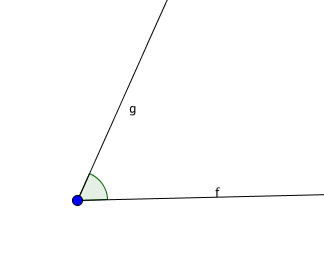
\includegraphics[scale=0.4]{definitions/angle.png}
\end{figure}
\end{definition}
\begin{definition}{Droite:}
Objet fondamental de la géométrie qui est indéfinissable. Mais l'on pourrait dire que c'est le plus court chemin pour rejoindre deux points infiniment éloignés, ou que c'est le chemin que suit la lumière dans un milieu homogène.
\end{definition}
\begin{definition}{Segment:}
Portion d'une droite
\end{definition}
\begin{definition}{Milieu:}
Point à égale distance des deux extrémités d'un segment
\end{definition}
\begin{definition}{Equidistant:}
A même distance, (du latin "aequidistans", "parallèle")
\end{definition}
\begin{definition}{Sécant:}
Qui se croise en un point unique
\end{definition}
\begin{definition}{Angle droit:}
Quart d'un tour
\end{definition}
\begin{definition}{Triangle:}
Réunion de trois points non alignés
\end{definition}
\begin{definition}{Cercle: }
Lieu géométrique à égale distance d'un point
\end{definition}
\begin{definition}{Parallèles:}
Deux droites qui ne se croisent qu'à l'infini, c'est à dire qui ne se croisent pas. (Du latin "parallelus", "parallèle")
\end{definition}
\begin{definition}{Perpendiculaires:}
Deux droites séparées par un angle égal à un quart de tour
\end{definition}
\begin{definition}{Médiatrice:}\label{def:mediatrice}
Droite perpendiculaire à un segment et qui partage celui-ci en deux parties isométriques
\end{definition}
\begin{definition}{Bissectrice:}
Ensemble des points équidistants à deux segments formant un angle, ou à deux droites sécantes
\end{definition}
\begin{definition}{Médiane:}
Droite passant par le sommet d'un triangle et qui passe par le milieu du côté qui y est opposé
\end{definition}
\begin{definition}{Hauteur:}
Droite passant pas l'un des sommets d'un triangle et qui est perpendiculaire au côté qui y est opposé
\end{definition}
\begin{definition}{Triangle isocèle:}
Triangle ayant deux côtés et deux angles isométriques
\end{definition}
\begin{definition}{Triangle équilatéral:}
Triangle dont les trois angles et les trois côtés sont isométriques, (du latin "aequilateralis", "équilatéral")
\end{definition}
\begin{definition}{Triangle rectangle:}
Triangle dont l'un des angles est droit
\end{definition}

%\end{document}